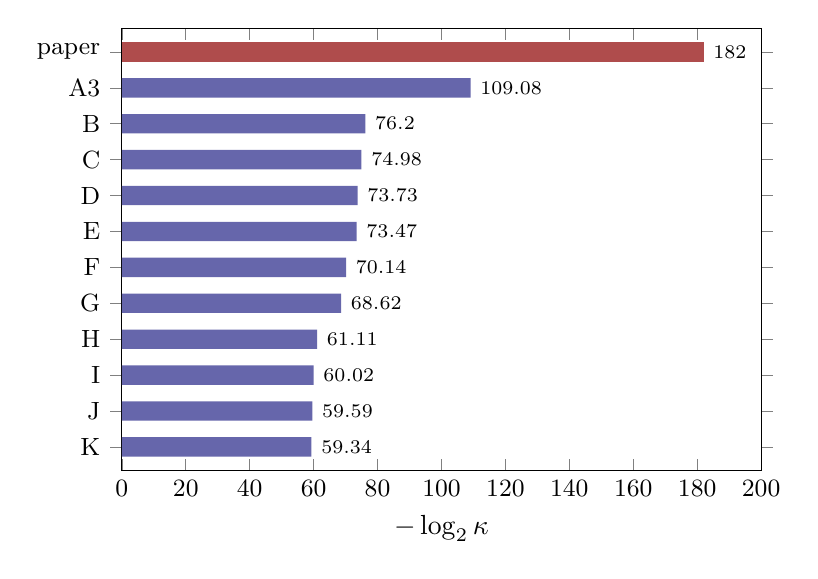
\begin{tikzpicture}
\begin{axis}[
  xbar, bar shift=0pt, width=0.8\textwidth, height=7.2cm,
  xmin=0, xmax=200,
  xlabel={$-\log_2 \kappa$},
  symbolic y coords={K,J,I,H,G,F,E,D,C,B,A3,paper},
  ytick={K,J,I,H,G,F,E,D,C,B,A3,paper}, y dir=normal,
  bar width=7pt,
  nodes near coords, nodes near coords align={horizontal},
  every node near coord/.append style={font=\scriptsize},
  enlarge y limits=0.06,
  tick label style={font=\small},
]
\addplot[fill=blue!45!black!60, draw=none] coordinates {
  (59.335,K) (59.591,J) (60.017,I) (61.114,H) (68.616,G) (70.142,F)
  (73.473,E) (73.733,D) (74.978,C) (76.199,B) (109.084,A3)
};
\addplot[fill=red!55!black!70, draw=none] coordinates {(182,paper)};
\end{axis}
\end{tikzpicture}
